\chapter{Begriffe und Ergänzungen}

\section{Aktionspotenzial}\label{appendix:aktionspotenzial}

\begin{figure}[h]
    \centering
    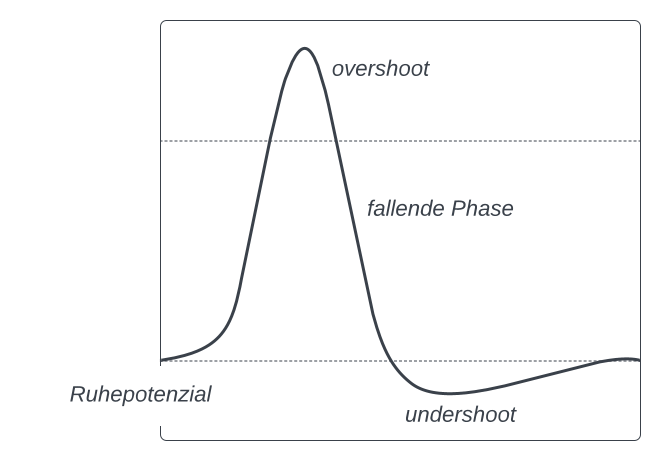
\includegraphics[
        width=12cm,
        keepaspectratio,
    ]{chapters/2. Das Neuron/images/aktionspotenzial_phasen}
    \caption{Phasen des Aktionspotenzials. (Quelle: in Anlehnung an~\cite[88, Abb. 4.1b]{BCP18})}
  \end{figure}

\subsubsection{Phasen des Aktionspotenzials}
Die Entstehung eines Aktionspotenzials kann entsprechend der zeitlichen Reihenfolge in folgende Phasen eingeteilt werden:

\subsubsection*{1. Aufstrich}
$Na^+$ gelangt in die Zelle,  $g_{Na}$  wird erhöht, mehr $Na+$ strömt ein (positiven Rückkoppelung).
Es kommt zu einer Depolarisation, $V_m$ wächst exponentiell (vgl.~\cite[46]{SD07}).

\subsubsection*{2. Overshoot}
$V_m$ wird positiv ($> 0 mV$) und nähert sich insgesamt $E_{Na} \sim 60 mV$ an\footnote{
    den es nicht erreicht. Erreicht werden Werte zwischen $0$ und $+40 mV$ (vgl.~\cite[69]{FE19})
} (vgl.~\cite[105]{BCP18}).

\subsubsection*{3. Repolarisationsphase}
Auch: Fallende Phase (vgl.~\cite[105]{BCP18}).
Natriumkanäle werden \textbf{inaktiviert}.
Spannungsabhängige Kaliumkanäle öffnen sich ca. $1 ms$ nach Depolarisation\footnote{
    vgl. ~\cite[105]{BCP18} und~\cite[47, Tafel 2.3 (A.2)]{SD07}
}, $K^+$-Ionen strömen aufgrund der elektrochemischen Triebkraft in den EZF, das Membranpotenzial wird wieder negativ\footnote{
    Die Kaliumleitfähigkeit wird ``verzögerter Gleichrichter`` genannt, da sie das ursprüngliche Membranpotenzial - mit Verzögerung - wiederherstellt (vgl.~\cite[103]{BCP18}).
}.


\subsubsection*{4. Undershoot\footnote{
    auch: ``Nachhyperpolarisation``~\cite[46]{SD07}
}}
Es kommt zu einem $V_m$, der unter $V_r$ liegt, da $g_{K}$ noch erhöht ist. $V_m$ nähert sich $E_k$ ($\sim-80 mV$), wozu auch eine erhöhte Pumprate der $Na^+$-$K^+$-ATPase\footnote{
    Die $Na^+$-$K^+$-ATPase ``erhält die Ionenkonzentrationsgradienten aufrecht, die für den Fluss von $Na^+$ und $K^+$ durch die Kanäle während des Aktionspotenzials erforderlich sind``(vgl.~\cite[105]{BCP18}).
} beitragen kann (vgl.~\cite[46]{SD07}).


\subsubsection*{5. Refraktärphase\footnote{
    Die Refraktärphase dient u.a. dazu, die Membran vor einer vorzeitigen Neuerregung zu schützen~\cite[76]{Jon19}.
    Hochfrequenten Aktionspotenzialsalven von max. 1000/s sind aufgrund dieser Eigenschaft möglich (vgl.~\cite[46]{SD07} sowie~\cite[89]{BCP18}).
    \textit{Bear et al.} stellen fest: ``Die Frequenz der Aktionspotenziale ist ein Maß für die Stärke des depolarisierenden Stroms``~\cite[89]{BCP18} - je stärker der Reiz, desto mehr Aktionspotenziale werden nacheinander abgefeuert (vgl.~\cite[90, Abb. 4.3]{BCP18}).
}}

- \textit{absolute}: Ca. 2 ms.
nach Auslösen des Aktionspotenzials sind die $Na^+$ Kanäle  \textit{inaktiviert} und dadurch nicht aktivierbar (vgl.~\cite[70]{FE19}).
Es ist keine Aktionspotenzialbildung möglich (vgl.~\cite[46]{SD07}).\\
- \textit{relative}: $V_m$ nähert sich weiter $V_r$ an.
Nachdem einige $Na^+$-Kanäle  \textit{deinaktiviert} wurden, ist eine Auslösung des Aktionspotenzials wieder möglich.
Allerdings ist die Reizschwelle erhöht (da $V_m < V_r < V_t$) und ``die Amplitude des auslösbaren Aktionspotenzials ist reduziert``~\cite[70]{FE19}.

\subsection{Übertragungsgeschwindigkeit von Signalen in Nervenzellen}
Ist das Axon - die Nervenfaser - \textbf{marklos} , wird das Signal kontinuierlich weitergeleitet, und die Leitunsggeschwindigkeit ist eher gering (ca. $1m/s$).
Die Leitunsggeschwindigkeit hängt hier direkt von dem Durchmesser der Nervenfaser ab und ist proportional zur Wurzel des Fasseradius.
Die marklosen Riesenaxone des Tintenfisches erreichen deshalb aufgrund ihrer Größe Leitungsgeschwindigkeiten von bis zu $20 m/s$ (vgl.~\cite[79]{Jon19}).

Im Gegensatz zu marklosen Nervenfasern erreichen \textbf{myelinisierte Axone} eine höhere Leitungsgeschwindigkeit.
Sie sind gegenüber ihrer Umgebung durch \textbf{Myelinscheiden}\footnote{
    Membranschichten, die sich bis zu 100 mal um das Axon wickeln (vgl.~\cite[79]{Jon19})
} besser isoliert (vgl.~\cite[48]{SD07}).
Dadurch wird der Stromfluss verstärkt und die Erregungsleitung erhöht sich.
Diese Isolierschicht ist ``segmentiert``: Myelinscheiden sind in Abständen von $0,2 - 2mm$ durch sog.  \textit{Ranvier-Schnürringe} unterbrochen.
Deren Membran besitzt spannungsabhängige $Na^+$-Kanäle, die das ankommende elektrische Signal durch  Depolarisierung der einzelnen Segmentabschnitte kontinuierlich weiterleiten - es wird an den Membranabschnitten jeweils ein neues Aktionspotenzial gebildet (vgl.~\cite[48]{SD07}).
Die Weiterleitung in myeliniserten Axonen bezeichnet man deshalb als \textbf{saltatorische} (sprunghafte) Erregungsleitung (vgl.~\cite[109 f.]{BCP18}).

\section{ATPasen}\label{appendix:atpasen}
Kurzform für \textit{Adenosintriphosphasen}: Enzyme, die ATP in ADP und Phosphat aufspalten (vgl.~\cite[26]{SD07}).

\section{Dendriten}\label{appendix:dendriten}
von ``\textgreek{δένδρον} (dendrón)`` (altgriechisch): Baum; einzelne selten länger als $2 mm$ (vgl.~\cite[28]{BCP18}).
Längere Dendriten finden sich an den kortikalen Pyramidenzellen mit einer Länge von $1 cm$ (vgl.~\cite[58]{Eil19}).

\section{Diffusion}\label{appendix:diffusion}
unter der Diffusion (``\textit{diffundere}`` (lat.): zerstreuen, ausbreiten) von Molekülen versteht man ihr Bestreben, entlang eines Konzentrationsgradienten (auch: Konzentrationsgefälles) einen Ausgleich der Konzentrationsunterschiede zu erreichen.
Moleküle in hoher Konzentration diffundieren dann in die Bereiche mit niedriger Konzentration: In den in Abschnitt~\ref{sec-ionenkonzentrationen} betrachteten Beispielen diffundieren bspw. $K^+$-Ionen, bis ein \textit{Gleichgewichtspotenzial} erreicht ist.

\section{Effektoren}
``efficere`` (lat.): bewirken, hervorbringen.
Effektoren können wir uns als Endglied der Signalübertragung vorstellen, auch wenn hier wieder interzelluläre Vorgänge stattfinden. Vgl. ``neuromuskuläre Endplatte`` in ~\cite[127, Abs. 3]{BCP18}.

\section{Expertensysteme}\label{appendix:expertensystem}

1990 von \textit{Friedrich und Stumptner} als ``kommerziell erfolgreichste Teildisziplin der Artificial intelligence`` bezeichnet~\cite[14]{FS90}, und ebenda beschrieben als:

\blockquote[{~\cite[14]{FS90}}]{
    Ziel der Expertensysteme ist es, dem Anwender Wissen und Fertigkeiten zur Verfügung zu stellen, über die normalerweise nur speziell ausgebildete oder erfahrene Personen (Experten) verfügen.
}

\noindent
Im groben besteht ein Expertensystem aus einer domänenspezifischen \textit{Wissensbasis}, auf der ein \textit{Inferenzmotor} zum Finden von Antworten und Schlussfolgerungen operiert. \textit{Russel und Norvig} erklären, dass Expertensysteme

\blockquote[{\cite[737]{RN09}}]{
    optimale Entscheidungen empfehlen und dabei die Prioritäten des Benutzers sowie die verfügbaren Evidenzen berücksichtigen
}


\section{Goldman-Gleichung}\label{appendix:goldman}

Auch: \textbf{Goldman-Hodgkin-Katz-Gleichung} (GHK-Gleichung) nach David Eliot Goldman (1910 – 1998), Alan Lloyd Hodgkin(1914 - 1998) und Bernard Katz (1911 - 2003).\\

Wie wir in Abschnitt~\ref{sec-ionenkonzentrationen} gesehen haben, liegt $V_r$ zwischen $-70 mV$ und $- 90mV$. Wie kann man nun schließen, dass das Ruhepotenzial durch die Membranpermeabilität von $K^+$ bestimmt wird, wenn $V_r = -70 mV$, aber $E_K = -80 mV$, und die Membran auch noch für andere Ionen wie bspw. $Na^+$ selektiv permeabel ist\footnote{
    vgl. ~\cite[77]{BCP18} sowie~\cite[44]{SD07}: ``Warum ist $E_m$ weniger negativ als $E_K${?}``
}? \\
Wäre die Membran nur für $K^+$ permeabel, so läge $V_r$ sicher bei $E_k$ (vgl.~\cite[32]{SD07}): Die Nernst-Gleichung kann deshalb nur zur Bestimmung des Membranpotenzials genutzt werden, wenn die Membran nur für ein Ion permeabel ist.
Ansonsten ist der erhaltene Wert nur näherungsweise zu verstehen (vgl.~\cite[67]{FE19}).\\

Das Membranpotenzial kann auch unter Berücksichtigung mehrerer Ionen bestimmt werden: Ionenkanäle unterstützen einen \textit{passiven Transport} der Ionen zwischen EZF und IZF \textit{entlang} ihres Konzentrationsgefälles, während Ionenpumpen, die \textit{entgegen} des Konzentrationsgefälles arbeiten, \textit{aktiv transportieren} (vgl.~\cite[30]{Fro19})\footnote{
    hierfür wird metabolische Energie verbraucht (vgl.~\cite[31]{Fro19}).
}.
Ionenpumpen sind für die Ionenkonzentrationsgradienten und deren Aufrechterhaltung verantwortlich (vgl.~\cite[76]{BCP18})\footnote{
    es wird ein nicht unwesentlicher Teil von Energie zur Aufrechterhaltung dieser Gradienten verbraucht. Die Natrium-Kalium-Pumpe verbraucht laut \textit{Bear et al.} etwa $70$ \% der ATP-Menge, die das Gehirn benötigt (vgl.~\cite[76]{BCP18}).
}.
Um $V_m$ zu berechnen müssen die Ionen mitberücksichtigt werden, für die die Membran permeabel ist.
Dazu kann die \textbf{Goldman-Gleichung} genutzt werden\footnote{
    \textit{Silbernagl und Despopoulos} nutzen für die Bestimmung von $V_m$ die fraktionelle Leitfähgkeit der involvierten Ionen und rechnen $V_r = E_K \times f_K + E_{Na}  \times f_{Na} + E_{Cl}  \times f_{Cl}$ (vgl.~\cite[32, 1.21]{SD07})
}.

\textit{Kandel et al.} stellen hierzu fest, dass eine hohe Konzentration eines einzelnen Ions zusammen mit einer hohen Membranpermeabilität für dieses Ion auch einen größeren Beitrag für $V_r$ leistet:

\blockquote[{\cite[135]{KSJ+13}}]{
    when permeability to one ion is exceptionally high, the Goldman equation reduces to the Nernst equation for that ion.
}

\textit{Fakler und Eilers} weisen darauf hin,

\blockquote[{\cite[67]{FE19}}]{
    dass die Permeabilitäten in komplizierter Weise von der Membranspannung und den Ionenkonzentrationen {[...]} abhängen und sich meist nur näherungsweise bestimmen lassen.
}


\section{KI Winter}\label{appendix:kiwinter}

Der Begriff ``KI Winter`` wird in der Literatur mit unterschiedlichen Perioden während der Forschung und Förderung von KI in Zusammenhang gebracht.
In dem Kontext des im Abschnitt~\ref{kiwinter} erwähnten Lighthill Reports bezieht sich der Begriff auf die Periode nach 1973

\blockquote[Artificial intelligence at edinburgh university: A perspective\footnote{https://www.inf.ed.ac.uk/about/AIhistory.html, abgerufen 31.08.2023}]{
    Lighthill's report provoked a massive loss of confidence in AI by the academic establishment in the UK (and to a lesser extent in the US). It persisted for a decade - the so-called 'AI Winter'.
}

\noindent
\textit{Russell und Norvig} beziehen sich auf einen Zeitraum um/ nach 1988, in dem nach einer Phase von Investitionen in Milliardenhöhe in den Forschungszweig ``viele Unternehmen verschwanden, weil sie ihre außergewöhnlichen Versprechungen nicht halten konnten.``~\cite[48]{RN09}. Auf gleichen Zeitraum bezieht sich \textit{McCorduck} in~\cite[432]{Mcc04}; vgl. hierzu auch:

\blockquote[{\cite[656; Hervorhebung i.O.]{Gar19}}]{
    Dozens of expert systems companies and AI-focused hardware manufacturers failed \textit{en masse} as hype turned to disillusionment.
}



\section{LeNet}\label{appendix:lenet1}

\textit{LeCun et al.} weisen darauf hin, dass LeNet eine Erweiterung der von LeCun beschriebenen Architektur in~\cite{Cun89} ist (vgl.~\cite[544]{CBD+89}).

Spätere Iterationen von \textit{LeNet} durch \textit{LeNet-4} und \textit{LeNet-5}. Die Architektur von \textit{LeNet-5} wird später angemessen mit der in Mitte der 90er Jahre zur Verfügung stehenden Technologie skaliert:

\blockquote[{\cite[15]{CBBH98}}]{
    In 1989 a recognizer as complex as LeNet-5 would have required several weeks' of training, and more data than was available, and was therefore not even considered.
}
\noindent
Eingabedaten für Lenet-5 sind ein $32 \times 32$ Pixel grosses Bild, außerdem besitzt das Netz 7 Schichten (ohne Eingabeschicht) (\textit{LeNet-1}: 3 verborgene Schichten (vgl.~\cite[544]{CBD+89})).
Eine vollständige Beschreibung der eindrucksvollen Architektur findet sich in~\cite[7 f.]{CBBH98}

\section{Lernrate}
Die \textbf{Lernrate} ($\eta$,in der Literatur auch $\alpha$) ist der Koeffizient für die Gewichtsanpassungen in einem künstlichen Neuron.

Wie in Abschnitt~\ref{sec:lernregel} gesehen, berechnet die Lernregel die Gewichte auf Basis des \textit{Fehlers}, also der Differenz von $\text{erwartete Ausgabe}$ und $\text{tatsächliche Ausgabe}$: Ist in den Beispielen der Fehler $-1$, werden die Gewichte verringert, ist der Fehler $1$, werden die Gewichte erhöht.
Die Lernrate $\eta$ ist der Koeffizient für die Gewichtsanpassung, und wird auch \textit{Schrittweite} genannt (vgl.~\cite[93]{GBC18} und~\cite[172]{RN09}).

Üblicherweise liegt $\eta$ zwischen $0$ und $1$\footnote{
    vgl.~\cite[61]{Fau94}; außerdem: ``$\alpha$ [$\eta$] ist eine kleine Konstante``~\cite[172]{RN09}. Gleiche Stelle beleuchtet das Für und Wider kleiner und großer Werte von $\eta$; \textit{Salomon} weist in~\cite[173]{Sal90} darauf hin, dass eine geeignete Lernrate auch von der Aufgabenstellung abhängt.
}.



\section{Neurotransmitter und ihre Rezeptoren}\label{appendix:neurotransmitter}

Die Diffusion der Vesikel in den synaptischen Spalt dauert ca. $10$ – $100$µs, danach binden sich die Transmitter an die Rezeptoren der postsynaptischen Zelle (vgl.~\cite[96]{HS19a}), die das ``interzellulläre chemische Signal [...] in ein intrazelluläres Signal (eine Änderung des Membranpotenzials oder eine chemische Veränderung) in der postsynaptischen Zelle umwandeln``~\cite[123]{BCP18}.

Rezeptoren können hierbei \textit{ionotrop} oder \textit{metabotrop} sein: Inotrope Rezeptoren sind gleichzeitig auch Ionenkanäle und aktivieren sich, wenn ein bestimmter Transmitter an sie bindet (vgl.~\cite[109]{HS19b}).

Metabotrope Rezeptoren lösen intrazelluläre Stoffwechselvorgänge aus, und weitere Botenstoffe (sog. \textbf{second messenger}) können dann für eine Aktivierung von Ionenkanälen verantwortlich sein (vgl.~\cite[134]{RK18})\footnote{
    ``postsynaptische Verdichtung`` bei~\cite[123]{BCP18}
}.

Als Neurotransmitter spielen im zentralen Nervensystem vor allem die Aminosäuren \textit{Glutamat} (Glu, erregend), \textit{Gamma-Aminobuttersäure} (GABA, hemmend)\footnote{
    GABA: Gamma-Aminobuttersäure. Um den GABA-Spiegel zu erhöhen, kann bspw. \textit{Gabapentin} verabreicht werden (\url{https://www.aerzteblatt.de/archiv/20049/Neuropathien-Gabapentin-bremst-ueberaktive-Neurone}, abgerufen 01.08.2023): Es ist bei der Behandlung von Anfallsleiden wie der Epilepsie sowie bei Nervenschmerzen (Neuropathien) wirksam (\url{https://www.gelbe-liste.de/wirkstoffe/Gabapentin_21579}, abgerufen 01.08.2023)
} und Glycin (Gly, hemmend) eine Rolle. An neuromuskulären Endplatten vermittelt Amin \textit{Acetylcholin} (ACh, erregend)\footnote{siehe Anhang~\ref{appendix:loewi} zur Entdeckung von ACh}.

Schnelle Formen der synaptischen Übertragung dauern zwischen $2$ und $100ms$, langsame Übertragungen einige $100$ Millisekunden bis Minuten (vgl.~\cite[129 f.]{BCP18}). Transmitter werden oft zusammen mit Co-Transmittern ausgeschüttet, die die Erregungsübertragung modulieren (vgl.~\cite[52]{SD07}).\\

Ob ein exzitatorischer oder inhibitorischer Transmitter auch dieselbe Wirkung in der postsynaptische Zelle hervorruft, entscheidet sich bei den Rezeptoren(vgl.~\cite[109]{HS19b}). Als Beispiel sei das bereits oben erwähnte ACh genannt, das die Kontraktion des Herzens verlangsamt, bei der Skelettmuskulatur jedoch eine schnelle Depolarisation der Muskelfasern bewirkt (vgl.~\cite[137]{BCP18}).

Erregende und hemmende Synapsen kann man auch an ihrer Struktur erkennen: Asymmetrische oder \textit{Gray-Typ-I-Synapsen} sind auf der postsynaptischen Seite dicker als auf der präsynaptischen, bei gleicher Dimension der Membrandifferenzierungen spricht man von \textit{Gray-Typ-II-Synapsen}. Typ-I sind in der Regel exzitatorisch, Typ-II inhibitorisch (vgl.~\cite[127 u. 147]{BCP18}).


\section{Perzeptron}\label{appendix:perzeptron}
\subsection*{The Perceptron - A perceiving and recognizing automaton}
Das Forschungsprojekt ``\textit{Perceiving and Recognizing Automaton}`` beschreibt einen Apparat, der mittels einer Kamera geometrische Figuren erkennen und zuordnen kann (vgl.~\cite[3]{Ros57}).
Die Funktionen simuliert Rosenblatt zunächst auf einem IBM 704 Rechner\footnote{
    ausführlich beschrieben in~\cite{Ros60}
}, bevor  die Hardware Anfang der 60er Jahre als \textit{Mark 1 Perceptron} gebaut wird: 400 Cadmiumsulfid-Photozellen auf einem 20x20 großen Raster angeordnet - dem \textbf{S-System} (\textbf{S} = \textit{Sensory}) - leiten Signale an das \textbf{A-System} (\textbf{A} = \textit{Association}); dort werden sie registriert und ausgewertet, und schlussendlich über das \textbf{R-System} (\textbf{R} = \textit{Response}) ausgegeben (vgl.~\cite[4 f.]{Ros57},~\cite[389 f.]{Ros58} sowie~\cite[193, ``Frank Rosenblatt]{Bis06} und~\cite[196, Figure 4.8]{Bis06}).
Dabei lernt die Maschine im ersten Schritt durch die Unterstützung der Ingenieure, wie gegebene Formen zu interpretieren sind: Für aktivierte Photozellen wird die erwartete Ausgabe manuell festgelegt.
Die Verbindungen zwischen den \textbf{S}-, \textbf{A}- und \textbf{R}-Units erinnert nicht nur von der Namensgebung her an biologische Neuronen, auch deren Struktur und Verschaltung wird hier als Vorbild genommen (vgl.~\cite[4]{Ros62}).\\

Die \textbf{S}-Units konnten sowohl hemmende als auch erregende Signale in das \textbf{A}-System einspeisen.
Darüber hinaus war das \textbf{R}-System in der Lage, über Rückkoppelungen hemmende Signale an das \textbf{A}-System zu senden: Damit sollte verhindert werden, dass weitere \textbf{R}-Units aktiviert werden, die sich mit den bereits aktivierten Units gegenseitig ausschließen (vgl.~\cite[4 f.]{Ros57}).



\section{Shunting Inhibition}\label{appendix:shuntinginhibition}
\subsection*{Kurzschlusshemmung bei Neuronen}
Wenn ein Transmitter einer inhibitorischen Synapse $Cl^-$-Kanäle aktiviert, verschiebt sich das Membranpotenzial in Richtung $E_{Cl} \sim -65 mV$.
Ist das Membranpotenzial der Zelle $> -65 mV$, kann ein hyperpolarisierendes IPSP ausgelöst werden.
Wenn allerdings bereits $V_m = E_{Cl}$ ist\footnote{
    ``häufig bei für Chloridleitfähigen GABA Rezeptoren``~\cite[100]{HS19a}
}, wird kein ``sichtbares`` IPSP ausgelöst (vgl. ~\cite[145 f.]{BCP18}) - die $Cl^-$-Kanäle sind offen, aber es findet keine Nettoionenbewegung statt.
Eine Hemmung der Zelle kann aber trotzdem noch stattfinden, wenn bspw. ein distal liegende exzitatorische Synapse positive Ladungsströme verursacht, und die inhibitorische Synapse proximal zum Soma liegt, in Stromrichtung ausgehend von der exzitatorischen Synapse.

Der positive Ladungsstrom kommt dann an der inhibitorischen Synapse mit den geöffnet $Cl^-$-Kanälen an, und die Depolarisation durch das EPSP wird durch den Einfluss von $Cl^-$-Ionen (die $V_m$ wieder auf $V_{rev} = E_{Cl}$ bringen wollen) mitigiert.\\

Aus diesem Grund sind inhibitorische Synapsen oft proximal zum Soma zu finden (vgl.~\cite[231]{KSJ+13}).


\section{Soma}\label{appendix:soma}
von ``\textgreek{σῶμα} (sõma)`` (altgriechisch): Körper; auch \textit{Perikaryon}~\cite[58]{RK18}.
Bezeichnet den Zellkörper und das Stoffwechselzentrum des Neurons mit der eine Größe von ca. $20$ μm~\cite[29]{BCP18}.
Zum Vergleich: ein menschliches Haar hat einen Durchmesser von ca. $70$ μm, kleine Bakterien bis zu $20$ μm.


\section{Umkehrpotenzial}\label{appendix:umkehrpotenzial}
Wie wir bei der Entstehung des Aktionspotenzials (siehe Abschnitt~\ref{sec:aktionspotenzial}) gesehen haben, transportieren spannungsgesteuerte Ionenkanäle stets entlang des elektrochemischen Gradienten (vgl.~\cite[39]{Fak19}).
Im Folgenden sei die Membran zur Vereinfachung nur permeabel für ein Ion, es gelte weiterhin $V_m < E_{Ion}$: Die Stromrichtung für das Ion ist einwärts IZF. Ist die Triebkraft positiv wegen $V_m > E_{Ion}$, strömt das Ion auswärts EZF. Wenn allerdings

\begin{equation}
    V_m - E_{Ion} = 0
\end{equation}

dann gilt:

\begin{equation}
    V_m = E_{Ion}
\end{equation}

In diesem Fall entspricht die Membranspannung dem Gleichgewichtspotenzial des Ions - es findet keine Nettoionenbewegung statt.\\

Der Wert für $V_m$, bei dem die Differenz zwischen $V_m$ und $E_{Ion}$ bei $0$ liegt, wird das \textit{Umkehrpotenzial} $V_{rev}$ genannt, weil hier ein Vorzeichenwechsel stattfindet: Je nachdem, in welche Richtung sich $V_m$ ändert, ändert sich auch die Richtung des Stroms.
Für ionenspezifische Kanäle entspricht das \textit{Umkehrpotenzial} ihrem \textit{Gleichgewichtspotenzial} (vgl.~\cite[95 f.]{SBB+13}).\\

Sobald eine Membran permeabel für mehr als ein spezifisches Ion ist, muss nach \textit{Kandel et al.} die relative Leitfähigkeit der Membran für diese Ionen sowie deren Gleichgewichtspotenziale zur Bestimmung des Umkehrpotenzials berücksichtigt werden (vgl.~\cite[196, Box 9--1]{KSJ+13}).
Für die ACh-Rezeptoren an der motorischen Endplatte\footnote{
    chemische Synapse, die Erregungen an eine Muskelfaser weiterleitet (vgl.~\cite[56]{SD07})
}, die für $Na^+$ und $K^+$ permeabel sind, folgt damit, dass die Summe ihrer Ströme am Umkehrpotenzial $V_{rev} = 0$ sein muss:

\begin{equation}
    I_{Ka} + I_{Na} = 0
\end{equation}

Da der Membranstrom $I_{Ion}$ gleich dem Produkt der Membranleitfähigkeit und der elektrochemischen Triebkraft für dieses Ion ist (vgl.~\cite[93]{BCP18}), also

\begin{equation}
    I_{Ion} = g_{Ion}  (V_m - E_{Ion})
\end{equation}

liefert Ersetzen die Gleichung

\begin{equation}
    g_{Na}  (V_m - E_{Na}) = g_{K}  (V_m - E_{K})
\end{equation}

Da am Umkehrpotenzial $V_{rev} = V_m$ gilt, können wir $V_m$ durch $E_{rev}$ ersetzen und danach auflösen, was zur folgenden Gleichung führt (vgl.~\cite[196, Box 9-1]{KSJ+13}):

\begin{equation}
    E_{rev} = \begin{matrix}
                  E_{Na} \space * \space (g_{Na} \space / \space g_{K}) \space + \space E_{K}  \\ \hline
                  (g_{Na} \space / \space g_{K}) \space + 1
    \end{matrix}
\end{equation}

Die ACh-Rezeptoren haben an der Endplatte eine relative Leitfähigkeit für $Na^+:K^+$ von $1,8$, für die Gleichgewichtspotenziale gilt $E_{Na} = +55 mV$ und $E_{K} = -100 mV$; somit folgt nach Einsetzen $E_{rev} = 0mV$ (vgl.~\cite[100]{HS19a}).
Wenn nun das Membranpotenzial vor der Einwirkung von ACh $< 0mV$ ist, bewirkt ein Öffnen der Ionenkanäle einen Strom einwärts IZF, um $V_m$ auf $0$ zu bringen (Depolarisation); im umgekehrten Fall $V_m > 0$ fließen Ionen auswärts zu EZF, und es findet eine Hyperpolarisation statt (vgl. ~\cite[136, Exkurs 5.4]{BCP18}).\\


